% Created by tikzDevice version 0.12.6 on 2026-07-31 11:12:44
% !TEX encoding = UTF-8 Unicode
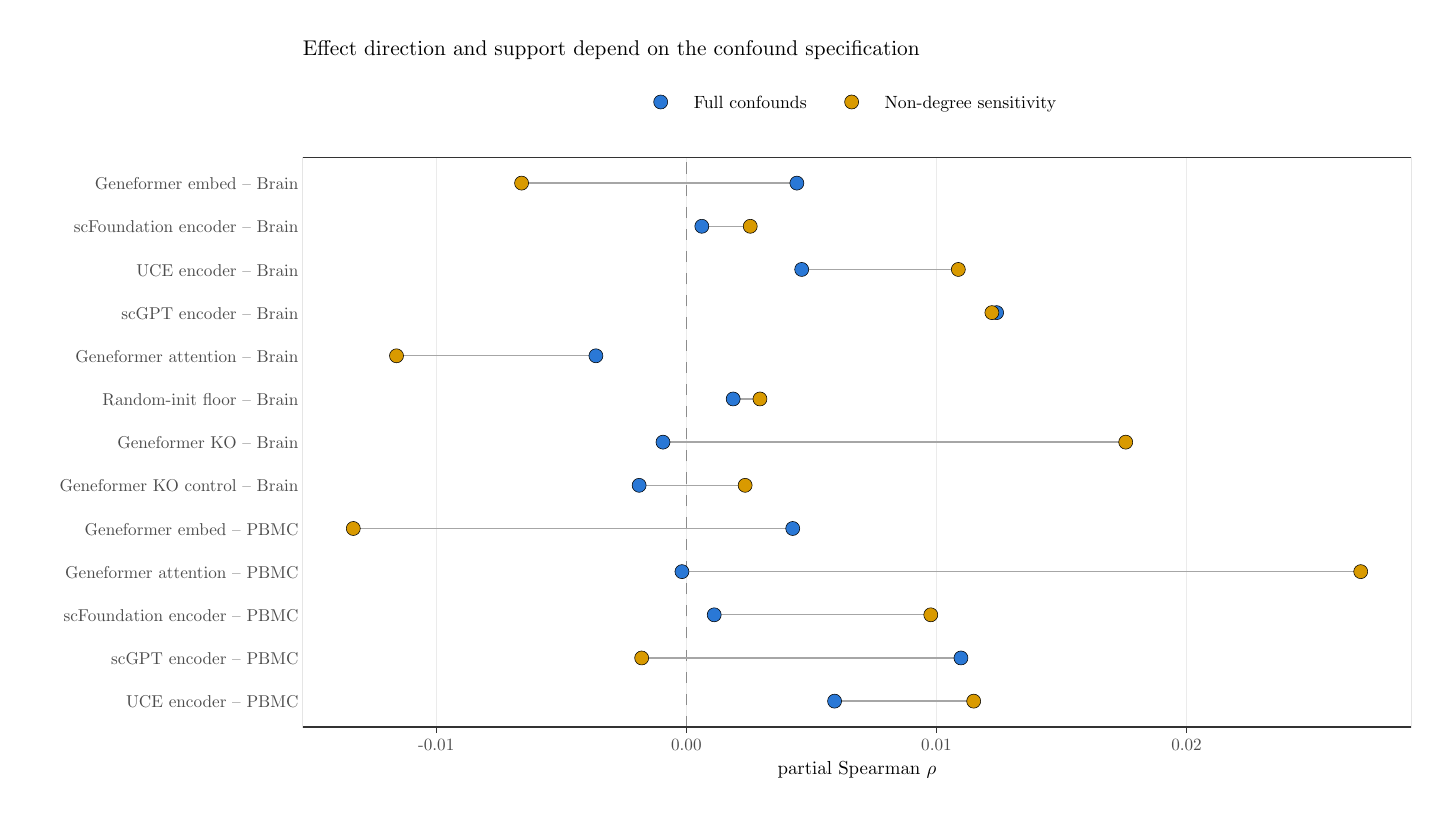
\begin{tikzpicture}[x=1pt,y=1pt]
\definecolor{fillColor}{RGB}{255,255,255}
\path[use as bounding box,fill=fillColor,fill opacity=0.00] (0,0) rectangle (505.89,274.63);
\begin{scope}
\path[clip] (  0.00,  0.00) rectangle (505.89,274.63);
\definecolor{drawColor}{RGB}{255,255,255}
\definecolor{fillColor}{RGB}{255,255,255}

\path[draw=drawColor,line width= 0.4pt,line join=round,line cap=round,fill=fillColor] (  0.00,  0.00) rectangle (505.89,274.63);
\end{scope}
\begin{scope}
\path[clip] ( 99.45, 21.91) rectangle (499.89,227.82);
\definecolor{fillColor}{RGB}{255,255,255}

\path[fill=fillColor] ( 99.45, 21.91) rectangle (499.89,227.82);
\definecolor{drawColor}{gray}{0.92}

\path[draw=drawColor,line width= 0.4pt,line join=round] (147.63, 21.91) --
	(147.63,227.82);

\path[draw=drawColor,line width= 0.4pt,line join=round] (238.01, 21.91) --
	(238.01,227.82);

\path[draw=drawColor,line width= 0.4pt,line join=round] (328.38, 21.91) --
	(328.38,227.82);

\path[draw=drawColor,line width= 0.4pt,line join=round] (418.75, 21.91) --
	(418.75,227.82);
\definecolor{drawColor}{gray}{0.55}

\path[draw=drawColor,line width= 0.4pt,dash pattern=on 4pt off 4pt ,line join=round] (238.01, 21.91) -- (238.01,227.82);
\definecolor{drawColor}{gray}{0.65}

\path[draw=drawColor,line width= 0.5pt,line join=round] (291.57, 31.27) --
	(341.84, 31.27);

\path[draw=drawColor,line width= 0.5pt,line join=round] (221.87, 46.87) --
	(337.24, 46.87);

\path[draw=drawColor,line width= 0.5pt,line join=round] (248.08, 62.47) --
	(326.33, 62.47);

\path[draw=drawColor,line width= 0.5pt,line join=round] (236.42, 78.07) --
	(481.69, 78.07);

\path[draw=drawColor,line width= 0.5pt,line join=round] (117.66, 93.66) --
	(276.45, 93.66);

\path[draw=drawColor,line width= 0.5pt,line join=round] (220.95,109.26) --
	(259.25,109.26);

\path[draw=drawColor,line width= 0.5pt,line join=round] (229.57,124.86) --
	(396.77,124.86);

\path[draw=drawColor,line width= 0.5pt,line join=round] (254.93,140.46) --
	(264.61,140.46);

\path[draw=drawColor,line width= 0.5pt,line join=round] (133.28,156.06) --
	(205.33,156.06);

\path[draw=drawColor,line width= 0.5pt,line join=round] (348.41,171.66) --
	(350.13,171.66);

\path[draw=drawColor,line width= 0.5pt,line join=round] (279.69,187.26) --
	(336.29,187.26);

\path[draw=drawColor,line width= 0.5pt,line join=round] (243.60,202.86) --
	(261.10,202.86);

\path[draw=drawColor,line width= 0.5pt,line join=round] (178.47,218.46) --
	(277.95,218.46);
\definecolor{drawColor}{RGB}{0,0,0}
\definecolor{fillColor}{RGB}{42,120,214}

\path[draw=drawColor,line width= 0.2pt,line join=round,line cap=round,fill=fillColor] (277.95,218.46) circle (  2.53);
\definecolor{fillColor}{RGB}{217,154,0}

\path[draw=drawColor,line width= 0.2pt,line join=round,line cap=round,fill=fillColor] (178.47,218.46) circle (  2.53);
\definecolor{fillColor}{RGB}{42,120,214}

\path[draw=drawColor,line width= 0.2pt,line join=round,line cap=round,fill=fillColor] (243.60,202.86) circle (  2.53);
\definecolor{fillColor}{RGB}{217,154,0}

\path[draw=drawColor,line width= 0.2pt,line join=round,line cap=round,fill=fillColor] (261.10,202.86) circle (  2.53);
\definecolor{fillColor}{RGB}{42,120,214}

\path[draw=drawColor,line width= 0.2pt,line join=round,line cap=round,fill=fillColor] (279.69,187.26) circle (  2.53);
\definecolor{fillColor}{RGB}{217,154,0}

\path[draw=drawColor,line width= 0.2pt,line join=round,line cap=round,fill=fillColor] (336.29,187.26) circle (  2.53);
\definecolor{fillColor}{RGB}{42,120,214}

\path[draw=drawColor,line width= 0.2pt,line join=round,line cap=round,fill=fillColor] (350.13,171.66) circle (  2.53);
\definecolor{fillColor}{RGB}{217,154,0}

\path[draw=drawColor,line width= 0.2pt,line join=round,line cap=round,fill=fillColor] (348.41,171.66) circle (  2.53);
\definecolor{fillColor}{RGB}{42,120,214}

\path[draw=drawColor,line width= 0.2pt,line join=round,line cap=round,fill=fillColor] (205.33,156.06) circle (  2.53);
\definecolor{fillColor}{RGB}{217,154,0}

\path[draw=drawColor,line width= 0.2pt,line join=round,line cap=round,fill=fillColor] (133.28,156.06) circle (  2.53);
\definecolor{fillColor}{RGB}{42,120,214}

\path[draw=drawColor,line width= 0.2pt,line join=round,line cap=round,fill=fillColor] (254.93,140.46) circle (  2.53);
\definecolor{fillColor}{RGB}{217,154,0}

\path[draw=drawColor,line width= 0.2pt,line join=round,line cap=round,fill=fillColor] (264.61,140.46) circle (  2.53);
\definecolor{fillColor}{RGB}{42,120,214}

\path[draw=drawColor,line width= 0.2pt,line join=round,line cap=round,fill=fillColor] (229.57,124.86) circle (  2.53);
\definecolor{fillColor}{RGB}{217,154,0}

\path[draw=drawColor,line width= 0.2pt,line join=round,line cap=round,fill=fillColor] (396.77,124.86) circle (  2.53);
\definecolor{fillColor}{RGB}{42,120,214}

\path[draw=drawColor,line width= 0.2pt,line join=round,line cap=round,fill=fillColor] (220.95,109.26) circle (  2.53);
\definecolor{fillColor}{RGB}{217,154,0}

\path[draw=drawColor,line width= 0.2pt,line join=round,line cap=round,fill=fillColor] (259.25,109.26) circle (  2.53);
\definecolor{fillColor}{RGB}{42,120,214}

\path[draw=drawColor,line width= 0.2pt,line join=round,line cap=round,fill=fillColor] (276.45, 93.66) circle (  2.53);
\definecolor{fillColor}{RGB}{217,154,0}

\path[draw=drawColor,line width= 0.2pt,line join=round,line cap=round,fill=fillColor] (117.66, 93.66) circle (  2.53);
\definecolor{fillColor}{RGB}{42,120,214}

\path[draw=drawColor,line width= 0.2pt,line join=round,line cap=round,fill=fillColor] (236.42, 78.07) circle (  2.53);
\definecolor{fillColor}{RGB}{217,154,0}

\path[draw=drawColor,line width= 0.2pt,line join=round,line cap=round,fill=fillColor] (481.69, 78.07) circle (  2.53);
\definecolor{fillColor}{RGB}{42,120,214}

\path[draw=drawColor,line width= 0.2pt,line join=round,line cap=round,fill=fillColor] (248.08, 62.47) circle (  2.53);
\definecolor{fillColor}{RGB}{217,154,0}

\path[draw=drawColor,line width= 0.2pt,line join=round,line cap=round,fill=fillColor] (326.33, 62.47) circle (  2.53);
\definecolor{fillColor}{RGB}{42,120,214}

\path[draw=drawColor,line width= 0.2pt,line join=round,line cap=round,fill=fillColor] (337.24, 46.87) circle (  2.53);
\definecolor{fillColor}{RGB}{217,154,0}

\path[draw=drawColor,line width= 0.2pt,line join=round,line cap=round,fill=fillColor] (221.87, 46.87) circle (  2.53);
\definecolor{fillColor}{RGB}{42,120,214}

\path[draw=drawColor,line width= 0.2pt,line join=round,line cap=round,fill=fillColor] (291.57, 31.27) circle (  2.53);
\definecolor{fillColor}{RGB}{217,154,0}

\path[draw=drawColor,line width= 0.2pt,line join=round,line cap=round,fill=fillColor] (341.84, 31.27) circle (  2.53);
\definecolor{drawColor}{gray}{0.20}

\path[draw=drawColor,line width= 0.4pt,line join=round,line cap=round] ( 99.45, 21.91) rectangle (499.89,227.82);
\end{scope}
\begin{scope}
\path[clip] (  0.00,  0.00) rectangle (505.89,274.63);
\definecolor{drawColor}{gray}{0.30}

\node[text=drawColor,anchor=base east,inner sep=0pt, outer sep=0pt, scale=  0.62] at ( 97.85, 28.86) {UCE encoder -- PBMC};

\node[text=drawColor,anchor=base east,inner sep=0pt, outer sep=0pt, scale=  0.62] at ( 97.85, 44.46) {scGPT encoder -- PBMC};

\node[text=drawColor,anchor=base east,inner sep=0pt, outer sep=0pt, scale=  0.62] at ( 97.85, 60.06) {scFoundation encoder -- PBMC};

\node[text=drawColor,anchor=base east,inner sep=0pt, outer sep=0pt, scale=  0.62] at ( 97.85, 75.65) {Geneformer attention -- PBMC};

\node[text=drawColor,anchor=base east,inner sep=0pt, outer sep=0pt, scale=  0.62] at ( 97.85, 91.25) {Geneformer embed -- PBMC};

\node[text=drawColor,anchor=base east,inner sep=0pt, outer sep=0pt, scale=  0.62] at ( 97.85,106.85) {Geneformer KO control -- Brain};

\node[text=drawColor,anchor=base east,inner sep=0pt, outer sep=0pt, scale=  0.62] at ( 97.85,122.45) {Geneformer KO -- Brain};

\node[text=drawColor,anchor=base east,inner sep=0pt, outer sep=0pt, scale=  0.62] at ( 97.85,138.05) {Random-init floor -- Brain};

\node[text=drawColor,anchor=base east,inner sep=0pt, outer sep=0pt, scale=  0.62] at ( 97.85,153.65) {Geneformer attention -- Brain};

\node[text=drawColor,anchor=base east,inner sep=0pt, outer sep=0pt, scale=  0.62] at ( 97.85,169.25) {scGPT encoder -- Brain};

\node[text=drawColor,anchor=base east,inner sep=0pt, outer sep=0pt, scale=  0.62] at ( 97.85,184.85) {UCE encoder -- Brain};

\node[text=drawColor,anchor=base east,inner sep=0pt, outer sep=0pt, scale=  0.62] at ( 97.85,200.45) {scFoundation encoder -- Brain};

\node[text=drawColor,anchor=base east,inner sep=0pt, outer sep=0pt, scale=  0.62] at ( 97.85,216.04) {Geneformer embed -- Brain};
\end{scope}
\begin{scope}
\path[clip] (  0.00,  0.00) rectangle (505.89,274.63);
\definecolor{drawColor}{gray}{0.20}

\path[draw=drawColor,line width= 0.4pt,line join=round] (147.63, 19.91) --
	(147.63, 21.91);

\path[draw=drawColor,line width= 0.4pt,line join=round] (238.01, 19.91) --
	(238.01, 21.91);

\path[draw=drawColor,line width= 0.4pt,line join=round] (328.38, 19.91) --
	(328.38, 21.91);

\path[draw=drawColor,line width= 0.4pt,line join=round] (418.75, 19.91) --
	(418.75, 21.91);
\end{scope}
\begin{scope}
\path[clip] (  0.00,  0.00) rectangle (505.89,274.63);
\definecolor{drawColor}{gray}{0.30}

\node[text=drawColor,anchor=base,inner sep=0pt, outer sep=0pt, scale=  0.62] at (147.63, 13.49) {-0.01};

\node[text=drawColor,anchor=base,inner sep=0pt, outer sep=0pt, scale=  0.62] at (238.01, 13.49) {0.00};

\node[text=drawColor,anchor=base,inner sep=0pt, outer sep=0pt, scale=  0.62] at (328.38, 13.49) {0.01};

\node[text=drawColor,anchor=base,inner sep=0pt, outer sep=0pt, scale=  0.62] at (418.75, 13.49) {0.02};
\end{scope}
\begin{scope}
\path[clip] (  0.00,  0.00) rectangle (505.89,274.63);
\definecolor{drawColor}{RGB}{0,0,0}

\node[text=drawColor,anchor=base,inner sep=0pt, outer sep=0pt, scale=  0.68] at (299.67,  4.66) {partial Spearman $\rho$};
\end{scope}
\begin{scope}
\path[clip] (  0.00,  0.00) rectangle (505.89,274.63);
\definecolor{fillColor}{RGB}{255,255,255}

\path[fill=fillColor] (216.79,235.82) rectangle (382.56,259.71);
\end{scope}
\begin{scope}
\path[clip] (  0.00,  0.00) rectangle (505.89,274.63);
\definecolor{fillColor}{RGB}{255,255,255}

\path[fill=fillColor] (220.79,239.82) rectangle (236.69,255.71);
\definecolor{drawColor}{RGB}{0,0,0}
\definecolor{fillColor}{RGB}{42,120,214}

\path[draw=drawColor,line width= 0.2pt,line join=round,line cap=round,fill=fillColor] (228.74,247.77) circle (  2.53);
\end{scope}
\begin{scope}
\path[clip] (  0.00,  0.00) rectangle (505.89,274.63);
\definecolor{fillColor}{RGB}{255,255,255}

\path[fill=fillColor] (289.79,239.82) rectangle (305.69,255.71);
\definecolor{drawColor}{RGB}{0,0,0}
\definecolor{fillColor}{RGB}{217,154,0}

\path[draw=drawColor,line width= 0.2pt,line join=round,line cap=round,fill=fillColor] (297.74,247.77) circle (  2.53);
\end{scope}
\begin{scope}
\path[clip] (  0.00,  0.00) rectangle (505.89,274.63);
\definecolor{drawColor}{RGB}{0,0,0}

\node[text=drawColor,anchor=base west,inner sep=0pt, outer sep=0pt, scale=  0.64] at (240.69,245.28) {Full confounds};
\end{scope}
\begin{scope}
\path[clip] (  0.00,  0.00) rectangle (505.89,274.63);
\definecolor{drawColor}{RGB}{0,0,0}

\node[text=drawColor,anchor=base west,inner sep=0pt, outer sep=0pt, scale=  0.64] at (309.69,245.28) {Non-degree sensitivity};
\end{scope}
\begin{scope}
\path[clip] (  0.00,  0.00) rectangle (505.89,274.63);
\definecolor{drawColor}{RGB}{0,0,0}

\node[text=drawColor,anchor=base west,inner sep=0pt, outer sep=0pt, scale=  0.77] at ( 99.45,264.60) {Effect direction and support depend on the confound specification};
\end{scope}
\end{tikzpicture}
